% beamer for weekly report
% Created by Zihan on 2023-06-22

% turn off sans-serif math
\documentclass[11pt]{beamer}

% Packages
% \Sum
\usepackage{amsmath}
% \coloneqq
\usepackage{mathtools}
% bookmark
\usepackage{bookmark}

% theme
\usetheme{default}
\usefonttheme{serif}

% title
\title{Weekly Report}

% author
\author{Zihan}

% date
\date{\today}

% Document
\begin{document}

% no title frame

% first page
% Talk about the paper supervisor asked me to read

\begin{frame}
    \frametitle{Co-Clustering to Reveal Salient Facial Features for Expression Recognition}
    \begin{itemize}
        \item \textbf{Proposal} Use co-clustering to select features that can be used to classify facial expressions
        \item \textbf{Idea}
              \begin{itemize}
                  \item Use Gabor filter to extract features vectors from facial images
                  \item Use co-cluster to build a relationship chain \\
                        Class $\stackrel{\text { label }}{\sim }$Samples $\stackrel{\text { co-cluster }}{\sim }$ Features
              \end{itemize}
        \item \textbf{Method}
              \begin{itemize}
                  \item Use Gabor filter to extract features from facial images
                  \item Use co-clustering to attain a subset of features and samples
                        % 计算每个co-cluster对应的samples和某个class契合的程度
                  \item Find the probability that a co-cluster is related to a certain class
                  \item Features with high probability are selected
              \end{itemize}
    \end{itemize}
\end{frame}
\begin{frame}
    \frametitle{Co-Clustering to Reveal Salient Facial Features for Expression Recognition}
    % insert a picture 'khan.png'
    \begin{figure}[htbp]
        \centering
        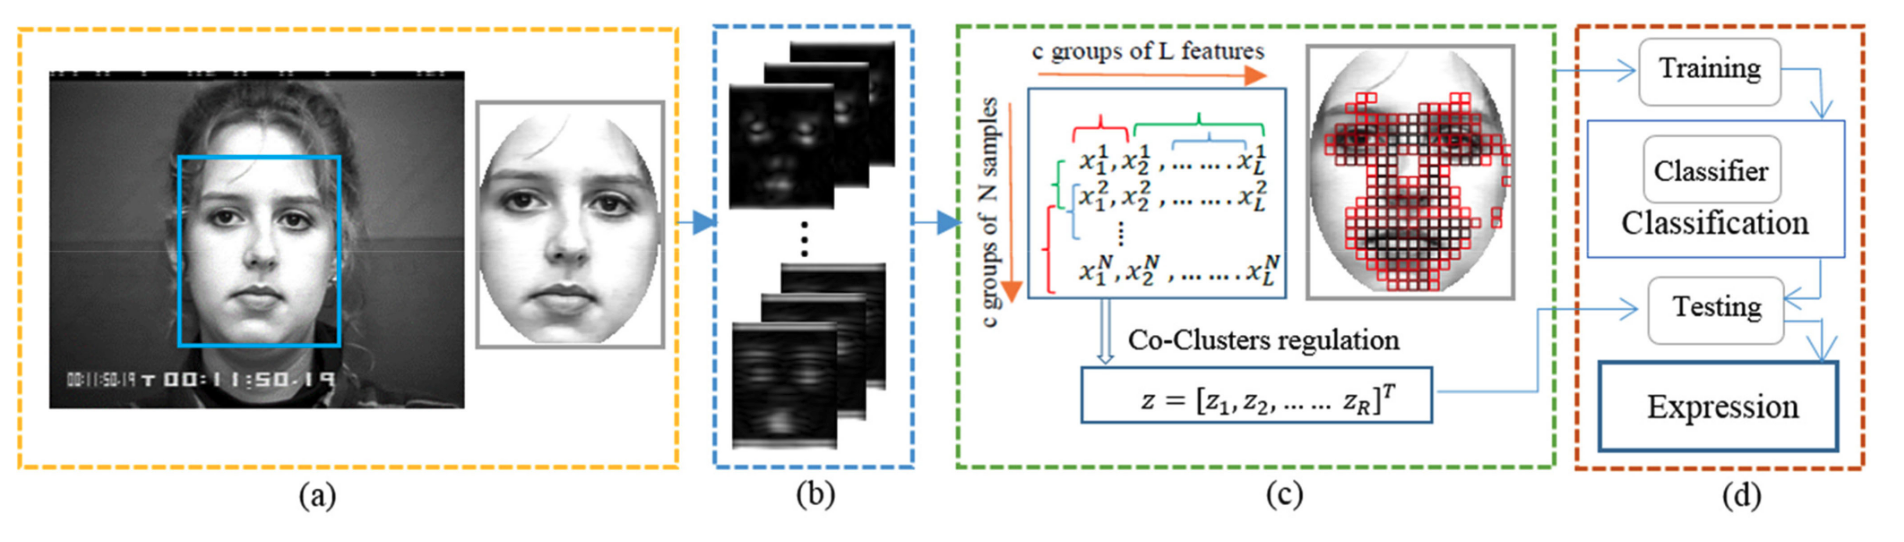
\includegraphics[width=\textwidth]{khan.png}
        % \caption{Khan et al. 2017}
    \end{figure}
    % insert a picture 'result.png'
    \begin{figure}[htbp]
        \centering
        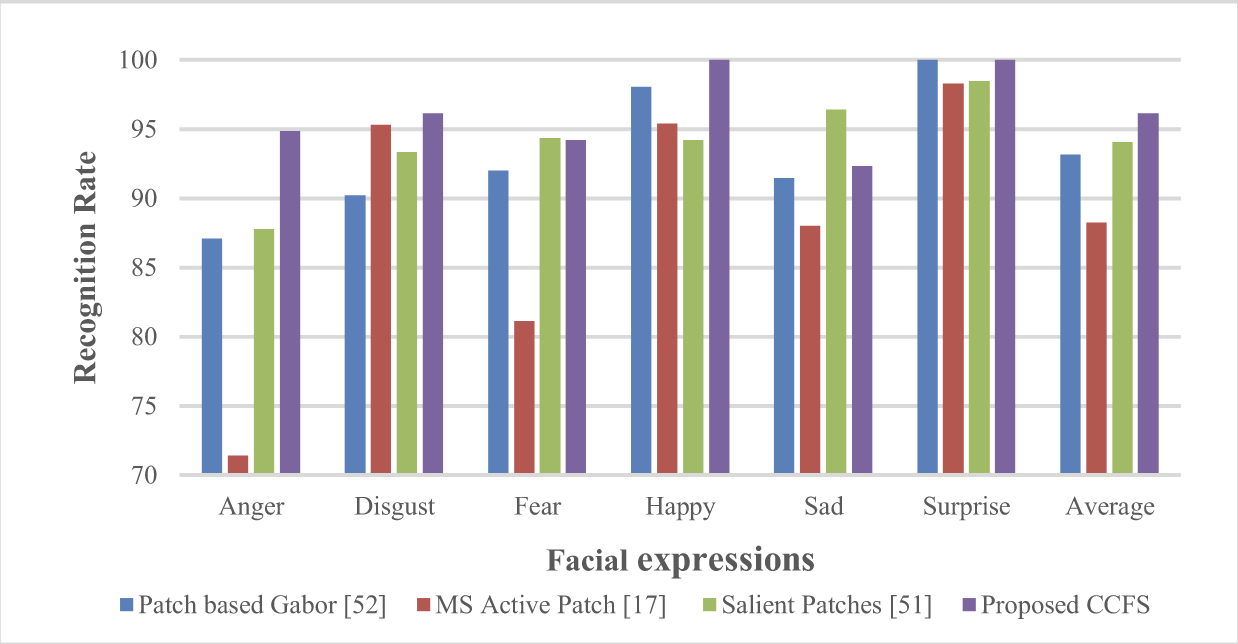
\includegraphics[width=0.6\textwidth]{result.png}
        % \caption{Result}
    \end{figure}
\end{frame}

% second page
% My proposal according to the paper

\begin{frame}
    \frametitle{My Proposal}
    \begin{itemize}
        \item \textbf{Proposal}: Use co-cluster to select features in NLP
        \item \textbf{Aims}: Use fewer features to get good prediction results, reducing the time and computational overhead of NLP training.
        \item \textbf{Method}:
              \begin{itemize}
                  \item Word-embedding or $n$-gram to extract features from text
                  \item (Maybe) Generate more features from the results above
                  \item Use co-clustering to attain a subset of features and samples
                  \item Select features that are related to a certain class most
              \end{itemize}

    \end{itemize}
    % insert mypro.jpeg
    \begin{figure}[htbp]
        \centering
        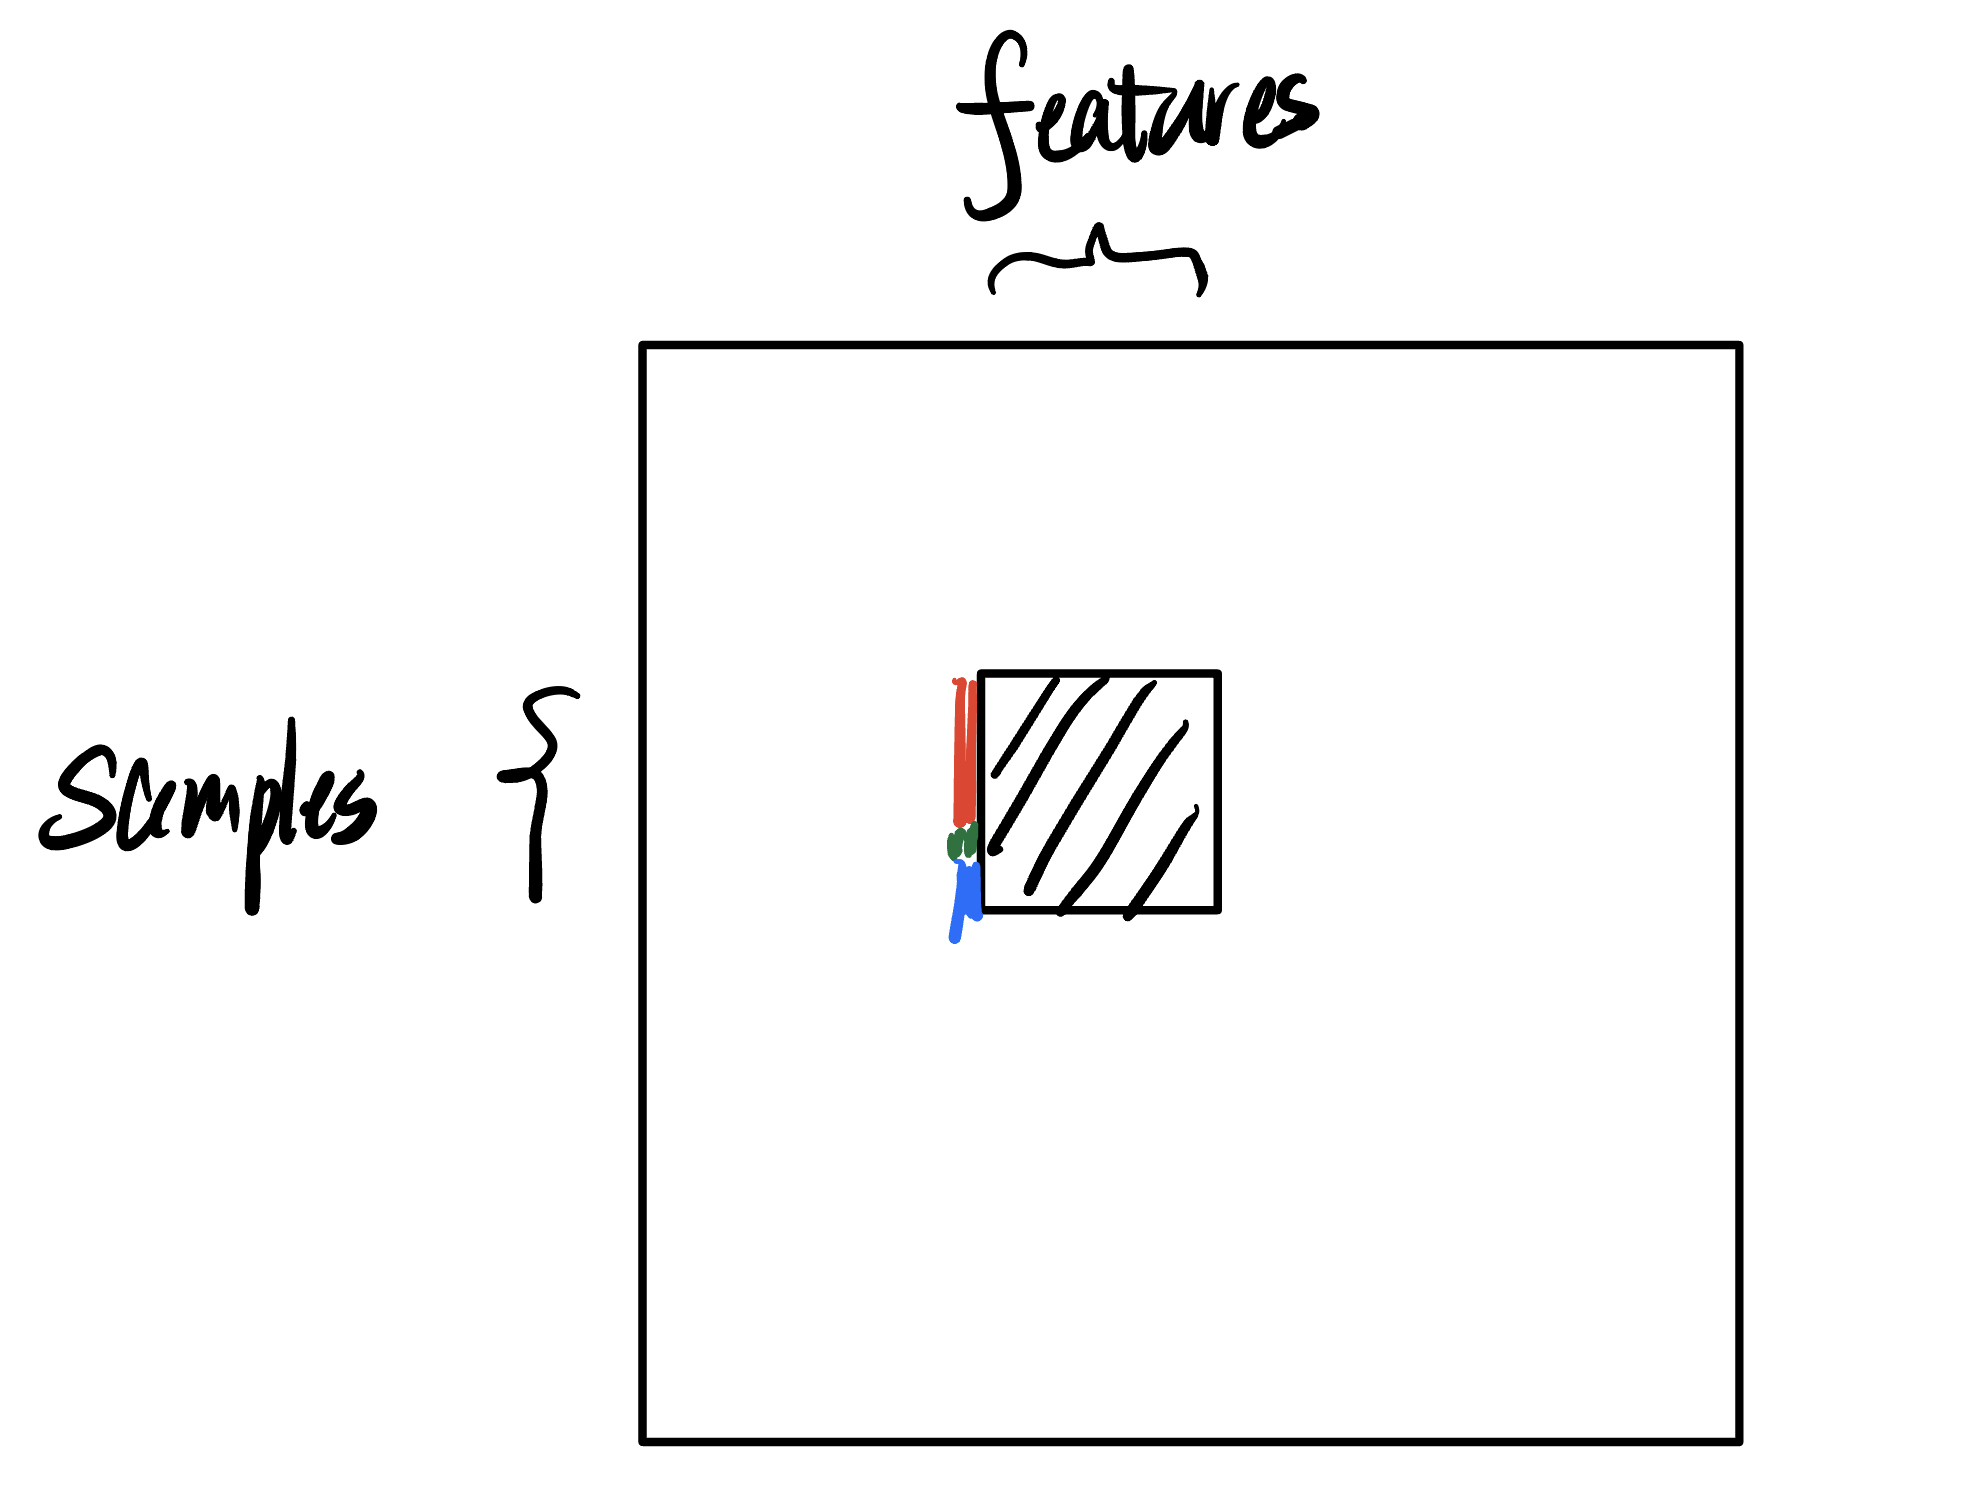
\includegraphics[width=0.4\textwidth]{mypro.jpeg}
        \caption{My Proposal, colors for classes}
    \end{figure}
\end{frame}

% third page
% I find another very high-quality paper about the feature selection in general case, which is 2017 best paper of ICML

\begin{frame}
    \frametitle{Understanding Black-box Predictions via Influence Functions (ICML 2017 Best Paper)}
    % Proposal: Influence function measures the impact of training data on the model - selection features
    % Methods:
    % 1) Influence function of samples on model parameters: Formula 1
    % 2) The influence function of samples on loss: Formula 2
    % 3) The influence function of samples on the selection of features: formula 3
    % Discussion: Different methods (co-cluster & influence function) for the same aims, need performance comparison

    \begin{itemize}
        \item \textbf{Proposal}: Influence function measures the impact of training data on the model - selection features
        \item \textbf{Method}:
              \begin{itemize}
                  \item Influence function of samples on model parameters: Formula 1
                  \item The influence function of samples on loss: Formula 2
                  \item The influence function of samples on the selection of features: formula 3
              \end{itemize}
        \item \textbf{Discussion}: Different methods (co-cluster \& influence function) for the same aims, need performance comparison
    \end{itemize}
    % \tiny
    % \begin{align*}
    %     z_\delta \stackrel{\text{def}}{=} (x+\delta, y), \quad
    %     \hat{\theta}_{\epsilon, z} \stackrel{\text{def}}{=}& \arg\min_{\theta\in\Theta} \frac{1}{n} \sum_{i=1}^n L(z_i, \theta) + \epsilon L(z, \theta)                                               \\
    %     \hat{\theta}_{\epsilon, z_\delta,-z} \stackrel{\text{def}}{=}& \arg\min_{\theta\in\Theta} \frac{1}{n} \sum_{i=1}^n L(z_i, \theta) + \epsilon L(z_\delta, \theta) - \epsilon L(z, \theta)      \\
    %     \mathcal{I}_{\text{up,params}}(z) \stackrel{\text{def}}{=} & \frac{d\hat{\theta}_{\epsilon, z}}{d\epsilon}\left.\right|_{\epsilon=0} = -H_{\hat{\theta}}^{-1} \nabla_\theta L(z, \hat{\theta}) \\
    %     \mathcal{I}_{\text{pert,loss}}(z, z_{\text{test}})^{\top} \stackrel{\text{def}}{=}& \left.\nabla_\delta L(z_{\text{test}}, \hat{\theta}_{z_\delta,-z})^{\top}\right|_{\delta=0} \\ =& -\nabla_\theta L(z_{\text{test}}, \hat{\theta})^{\top} H_{\hat{\theta}}^{-1} \nabla_x \nabla_\theta L(z, \hat{\theta})
    % \end{align*}

    % \begin{small}
    %     \begin{align*}
    %         z_\delta \stackrel{\text{def}}{=} (x+\delta, y), \quad
    %         \hat{\theta}_{\epsilon, z} \stackrel{\text{def}}{=}& \arg\min_{\theta\in\Theta} \frac{1}{n} \sum_{i=1}^n L(z_i, \theta) + \epsilon L(z, \theta)                                               \\
    %         \hat{\theta}_{\epsilon, z_\delta,-z} \stackrel{\text{def}}{=}& \arg\min_{\theta\in\Theta} \frac{1}{n} \sum_{i=1}^n L(z_i, \theta) + \epsilon L(z_\delta, \theta) - \epsilon L(z, \theta)      \\
    %         \left.\mathcal{I}_{\text{up,params}}(z) \stackrel{\text{def}}{=}& \frac{d\hat{\theta}_{\epsilon, z}}{d\epsilon}\right|_{\epsilon=0} = -H_{\hat{\theta}}^{-1} \nabla_\theta L(z, \hat{\theta}) \\
    %         \mathcal{I}_{\text{pert,loss}}(z, z_{\text{test}})^{\top} \stackrel{\text{def}}{=}& \left.\nabla_\delta L(z_{\text{test}}, \hat{\theta}_{z_\delta,-z})^{\top}\right|_{\delta=0} = -\nabla_\theta L(z_{\text{test}}, \hat{\theta})^{\top} H_{\hat{\theta}}^{-1} \nabla_x \nabla_\theta L(z, \hat{\theta})
    %     \end{align*}
    % \end{small}

    % $$
    %     z_\delta \stackrel{\text { def }}{=}(x+\delta, y),
    %     \hat{\theta}_{\epsilon, z} \stackrel{\text { def }}{=} \arg \min _{\theta \in \Theta} \frac{1}{n} \sum_{i=1}^n L\left(z_i, \theta\right)+\epsilon L(z, \theta)
    % $$
    % $$
    %     \hat{\theta}_{\epsilon, z_\delta,-z} \stackrel{\text { def }}{=}\arg \min _{\theta \in \Theta} \frac{1}{n} \sum_{i=1}^n L\left(z_i, \theta\right)+\epsilon L\left(z_\delta, \theta\right)-\epsilon L(z, \theta)
    % $$
    % $$
    %     \left.\mathcal{I}_{\text {up,params }}(z) \stackrel{\text { def }}{=} \frac{d \hat{\theta}_{\epsilon, z}}{d \epsilon}\right|_{\epsilon=0}=-H_{\hat{\theta}}^{-1} \nabla_\theta L(z, \hat{\theta})
    % $$
    % $$
    %     \begin{aligned}
    %         \mathcal{I}_{\text {pert,loss }}\left(z, z_{\text {test }}\right)^{\top} & \left.\stackrel{\text { def }}{=} \nabla_\delta L\left(z_{\text {test }}, \hat{\theta}_{z_\delta,-z}\right)^{\top}\right|_{\delta=0} \\
    %                                                                                  & =-\nabla_\theta L\left(z_{\text {test }}, \hat{\theta}\right)^{\top} H_{\hat{\theta}}^{-1} \nabla_x \nabla_\theta L(z, \hat{\theta})
    %     \end{aligned}
    % $$
\end{frame}

\begin{frame}
    \textbf{Method}:
    \begin{itemize}
        \item Influence function of samples on model parameters: Formula 1
        \item The influence function of samples on loss: Formula 2
        \item The influence function of samples on the selection of features: formula 3
    \end{itemize}
        \begin{align*}
            z_\delta \stackrel{\text{def}}{=} (x+\delta, y), \quad
            \hat{\theta}_{\epsilon, z} \stackrel{\text{def}}{=}& \arg\min_{\theta\in\Theta} \frac{1}{n} \sum_{i=1}^n L(z_i, \theta) + \epsilon L(z, \theta)                                               \\
            \hat{\theta}_{\epsilon, z_\delta,-z} \stackrel{\text{def}}{=}& \arg\min_{\theta\in\Theta} \frac{1}{n} \sum_{i=1}^n L(z_i, \theta) + \epsilon L(z_\delta, \theta) - \epsilon L(z, \theta)      \\
            \mathcal{I}_{\text{up,params}}(z) \stackrel{\text{def}}{=} & \frac{d\hat{\theta}_{\epsilon, z}}{d\epsilon}\left.\right|_{\epsilon=0} = -H_{\hat{\theta}}^{-1} \nabla_\theta L(z, \hat{\theta}) \\
            \mathcal{I}_{\text{pert,loss}}(z, z_{\text{test}})^{\top} \stackrel{\text{def}}{=}& \left.\nabla_\delta L(z_{\text{test}}, \hat{\theta}_{z_\delta,-z})^{\top}\right|_{\delta=0} \\ =& -\nabla_\theta L(z_{\text{test}}, \hat{\theta})^{\top} H_{\hat{\theta}}^{-1} \nabla_x \nabla_\theta L(z, \hat{\theta})
        \end{align*}

\end{frame}
% \begin{frame}
%     \frametitle{Understanding Black-box Predictions via Influence Functions (ICML 2017 Best Paper)}

%     \begin{columns}[T]
%         \begin{column}{0.5\textwidth}
%             \begin{itemize}
%                 \item \textbf{Proposal}: Influence function measures the impact of training data on the model - selection features
%                 \item \textbf{Method}:
%                       \begin{itemize}
%                           \item Influence function of samples on model parameters: Formula 1
%                           \item The influence function of samples on loss: Formula 2
%                           \item The influence function of samples on the selection of features: formula 3
%                       \end{itemize}
%                 % \item \textbf{Discussion}: Different methods (co-cluster \& influence function) for the same aims, need performance comparison
%             \end{itemize}
%         \end{column}
%         \begin{column}{0.5\textwidth}
%             \textbf{Discussion}: Different methods (co-cluster \& influence function) for the same aims, need performance comparison
%             \tiny
%             \begin{align*}
%                 z_\delta \stackrel{\text{def}}{=} (x+\delta, y), \quad
%                 \hat{\theta}_{\epsilon, z} \stackrel{\text{def}}{=}& \arg\min_{\theta\in\Theta} \frac{1}{n} \sum_{i=1}^n L(z_i, \theta) + \epsilon L(z, \theta)                                               \\
%                 \hat{\theta}_{\epsilon, z_\delta,-z} \stackrel{\text{def}}{=}& \arg\min_{\theta\in\Theta} \frac{1}{n} \sum_{i=1}^n L(z_i, \theta) + \epsilon L(z_\delta, \theta) - \epsilon L(z, \theta)      \\
%                 \mathcal{I}_{\text{up,params}}(z) \stackrel{\text{def}}{=} & \frac{d\hat{\theta}_{\epsilon, z}}{d\epsilon}\left.\right|_{\epsilon=0} = -H_{\hat{\theta}}^{-1} \nabla_\theta L(z, \hat{\theta}) \\
%                 \mathcal{I}_{\text{pert,loss}}(z, z_{\text{test}})^{\top} \stackrel{\text{def}}{=}& \left.\nabla_\delta L(z_{\text{test}}, \hat{\theta}_{z_\delta,-z})^{\top}\right|_{\delta=0} \\ =& -\nabla_\theta L(z_{\text{test}}, \hat{\theta})^{\top} H_{\hat{\theta}}^{-1} \nabla_x \nabla_\theta L(z, \hat{\theta})
%             \end{align*}
%         \end{column}
%     \end{columns}

% \end{frame}
\end{document}
